\item A horizontal smooth rod \( AB \) rotates with a constant angular velocity \( \omega = 2.00 \ \text{rad/s} \) about a vertical axis passing through its end \( A \). A freely sliding sleeve of mass \( m = 0.50 \ \text{kg} \) moves along the rod from the point \( A \) with the initial velocity \( v_0 = 1.00 \ \text{m/s} \). Find the Coriolis force acting on the sleeve (in the reference frame fixed to the rotating rod) at the moment when the sleeve is located at the distance \( r = 50 \ \text{cm} \) from the rotation axis.
    \begin{center}
        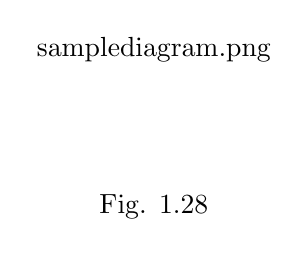
\begin{tikzpicture}
            \node at (0, 0) {{samplediagram.png}};
            \node at (0, -2) {Fig. 1.28};
        \end{tikzpicture}
    \end{center}